\section*{WU2}
The training accuracy goes down after increasing number of examples. This is because there would be more ambiguity, meaning there would be examples with different lables with same feature values at non-leaf nodes where the DT makes a decision.

The testing error could go down even after you increase the number of examples. This is because the features that are considered important on training phase can vary as the number of examples changes. Let's say, when there are 50 examples, a feature $x_{a1}$ is considered more dominant than the other features. However, as the number of examples increases, say 100, another feature $x_{a2}$ may be considered more influential than $x_{a1}$. This may be right or wrong on the test data. If it is right on test data, the test accuracy goes up, and vice versa.

\section*{WU3}
\begin{figure}[here]
	\caption{Plot of DT with various numbers of examples}
	\label{fig:dt_examples}
	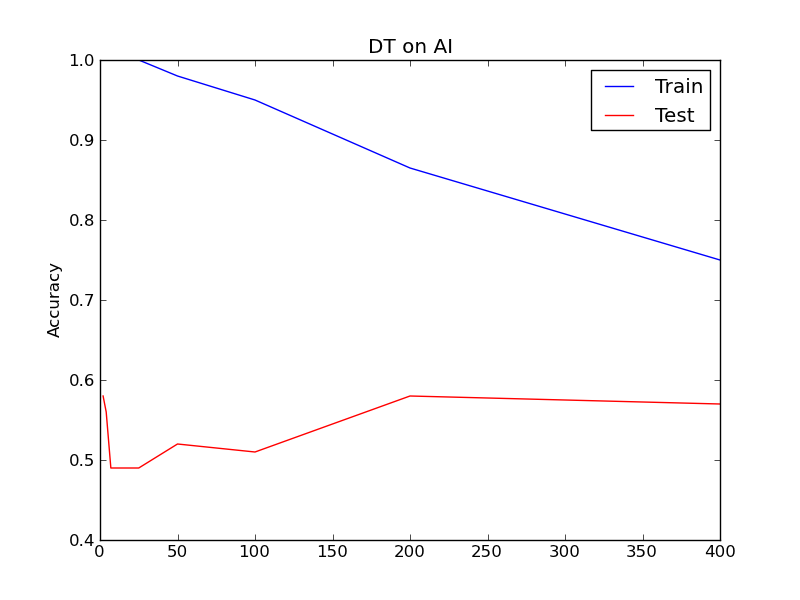
\includegraphics[width=6.5in]{images/dt_examples.png}
\end{figure}

Please refer to the figure \ref{fig:dt_examples}.

The training accuracy is guaranteed to monotonically increase, because it is table-look-up, except for the case which at every node on DT the probability of going right or left is 50-50. This will never increase the accuracy, but it is very unlikely to happen. 

The testing accuracy could oscillate like on the figure, but not guaranteed. As questions asked at DT nodes go up, the model tends to overfit. This could either increase or decrease in accuracy. However, in the end the accuracy goes down overall.

\section*{WU4}
\begin{figure}[here]
	\caption{Plot of DT with various depth parameters}
	\label{fig:dt_depth}
	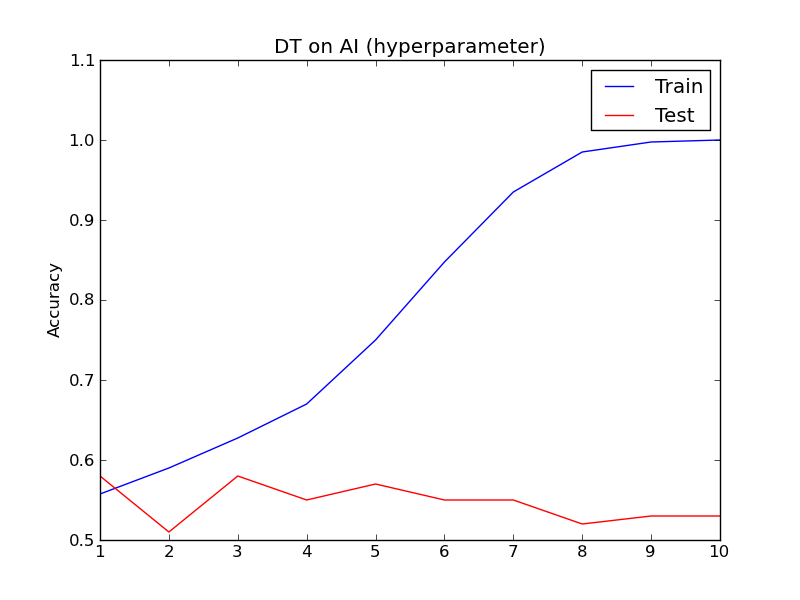
\includegraphics[width=6.5in]{images/dt_depth.png}
\end{figure}

Please refer to the figure \ref{fig:dt_depth}.
  \begin{verbatim}
-introduction to low-level programming concepts [212]
   - program analysis and understanding [631]
     - computer processing of pictorial information [733]
       - Leaf -1.0
       - Leaf 1.0
     - introduction to human-computer interaction [434]
       - Leaf -1.0
       - Leaf 1.0
   - computational linguistics ii [773]
     - computational methods [460]
       - Leaf -1.0
       - Leaf 1.0
     - computational geometry [754]
       - Leaf 1.0
       - Leaf 1.0
  \end{verbatim}
I may be wrong and there may be correlation between taking CG and taking these courses, but the courses look fairly random to me. This implies DT is not the best model for this problem.

